%%%%%%%%%%%%%%%%%%%%%%%%%%%%%%%%%%%%%%%%%
% baposter Portrait Poster
% LaTeX Template
% Version 1.0 (15/5/13)
%
% Created by:
% Brian Amberg (baposter@brian-amberg.de)
%
% This template has been downloaded from:
% http://www.LaTeXTemplates.com
%
% License:
% CC BY-NC-SA 3.0 (http://creativecommons.org/licenses/by-nc-sa/3.0/)
%
%%%%%%%%%%%%%%%%%%%%%%%%%%%%%%%%%%%%%%%%%

%----------------------------------------------------------------------------------------
%	PACKAGES AND OTHER DOCUMENT CONFIGURATIONS
%----------------------------------------------------------------------------------------

\documentclass[a0paper,portrait]{baposter}

\usepackage[font=small,labelfont=bf]{caption} % Required for specifying captions to tables and figures
\usepackage{booktabs} % Horizontal rules in tables
\usepackage{relsize} % Used for making text smaller in some places
\usepackage{amsmath}
\usepackage{amssymb}
\usepackage{amsfonts}
\usepackage{xparse}
\usepackage{physics}
\usepackage{esint}
\usepackage{bbold}
\usepackage{cite}
\usepackage{tikz}

\graphicspath{{figures/}} % Directory in which figures are stored

\definecolor{bordercol}{RGB}{40,40,40} % Border color of content boxes
\definecolor{headercol1}{RGB}{186,215,230} % Background color for the header in the content boxes (left side)
\definecolor{headercol2}{RGB}{80,80,80} % Background color for the header in the content boxes (right side)
\definecolor{headerfontcol}{RGB}{0,0,0} % Text color for the header text in the content boxes
\definecolor{boxcolor}{RGB}{255,255,255} % Background color for the content in the content boxes



\begin{document}

\background{ % Set the background to an image (background.pdf)
\begin{tikzpicture}[remember picture,overlay]
\draw (current page.north west)+(-2em,2em) node[anchor=north west]
{
\includegraphics[height=1.1\textheight]{background.pdf}};
\end{tikzpicture}
}

\begin{poster}{
grid=false,
borderColor=bordercol, % Border color of content boxes
headerColorOne=headercol1, % Background color for the header in the content boxes (left side)
headerColorTwo=headercol2, % Background color for the header in the content boxes (right side)
headerFontColor=headerfontcol, % Text color for the header text in the content boxes
boxColorOne=boxcolor, % Background color for the content in the content boxes
headershape=smallrounded, % Specify the rounded corner in the content box headers
headerfont=\Large\sf\bf, % Font modifiers for the text in the content box headers
textborder=rectangle,
background=user,
headerborder=closed, % Change to closed for a line under the content box headers
boxshade=plain
}
{}
%
%----------------------------------------------------------------------------------------
%	TITLE AND AUTHOR NAME
%----------------------------------------------------------------------------------------
%
{\vspace{-8pt}\sf\bf Geometry and Spin Transport \\ \vspace{8pt}in Skyrmion Magnets} % Poster title
{\begin{minipage}[t]{0.4\textwidth} \smaller
		Researcher: Benjamin Brown \\
		Benjamin.Brown@Warwick.ac.uk
\end{minipage}
\qquad
\begin{minipage}[t]{0.4\textwidth} \smaller
	Supervisor: Dr. Gareth Alexander \\
	G.P.Alexander@Warwick.ac.uk
\end{minipage}
\vspace{2mm}

{\smaller Department of Physics, University of Warwick, Coventry, United Kingdom}} % Author email addresses
{
\includegraphics[scale=0.35]{UofW.pdf}} % University/lab logo

%----------------------------------------------------------------------------------------
%	ABSTRACT
%----------------------------------------------------------------------------------------

\headerbox{Abstract}{name=introduction,column=0,row=0}{
We investigate the emergent electrodynamic fields that arise from potentials when a free electron travels through a skyrmion magnetic texture. In the adiabatic limit we project these potentials onto the spin axis, allowing us to investigate the nature of the emergent fields. We consider the cases where the magnetic texture is time-independent and time-dependent, and find that a spin-motive force makes itself manifest.

}

%----------------------------------------------------------------------------------------
%	INTRODUCTION
%----------------------------------------------------------------------------------------

\headerbox{Introduction}{name=methods,column=0,below=introduction}{

The equilibrium magnetisation field in chiral magnets often possess a non-trivial topology. An example of such a configuration is the magnetic skyrmion, which is a vortex-like whirl found under certain conditions in transition metal compounds such as MnSi \cite{10.2307/20403069}.
\vspace{-8pt}
\begin{center}
	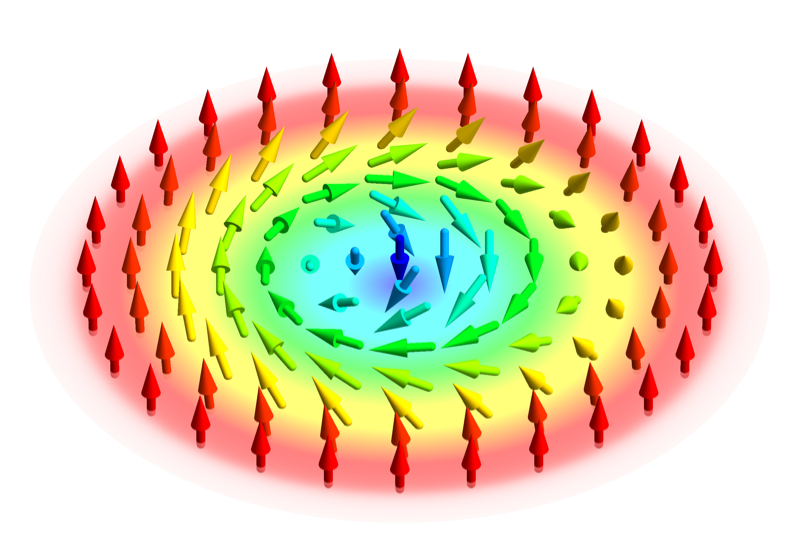
\includegraphics[width=0.49\linewidth]{skyrmion}
	\captionof{figure}[centering]{A vortex-like magnetic whirl, \textit{i.e.} a skyrmion \cite{Soccer}.}
\end{center}
An interesting consequence of the skyrmion texture is that it endows to the wavefunction of a free election travelling through the texture a geometric phase, which can be interpreted as a Lorentz force due to emergent electromagnetic fields \cite{Soccer}. The aim of this project is to describe the dynamics of these electrons due to these fields.
}

%----------------------------------------------------------------------------------------
%	CONCLUSION
%----------------------------------------------------------------------------------------

\headerbox{Conclusion}{name=conclusion,column=0,below=methods}{

We have described the emergent electromagnetic fields that arise when a free electron travels though a skyrmion magnetic texture. When a magnetic field is applied orthogonally to the basal plane, an emergent electric field arises which acts to deflect free electrons radially from the skyrmion core. 
To take this project further, it would be interesting to investigate:

\begin{enumerate}
\item How different forms of the LLG equation determine the emergent electric field.
\item The effect that non-adiabicity has on the potentials.
\end{enumerate}
}

%----------------------------------------------------------------------------------------
%	REFERENCES
%----------------------------------------------------------------------------------------

\headerbox{References}{name=references,column=0,below=conclusion}{

\smaller % Reduce the font size in this block
\renewcommand{\section}[2]{\vskip 0.05em} % Get rid of the default "References" section title
\nocite{*} % Insert publications even if they are not cited in the poster

\bibliographystyle{unsrt}
\bibliography{skyrmion} % Use sample.bib as the bibliography file
}

%----------------------------------------------------------------------------------------
%	ACKNOWLEDGEMENTS
%----------------------------------------------------------------------------------------

\headerbox{Acknowledgements}{name=acknowledgements,column=0,below=references, above=bottom}{

\smaller % Reduce the font size in this block
I would like to thank my supervisor Dr. Gareth Alexander for useful discussions, and for giving me the opportunity to pursue this project. This project was supported by the Undergraduate Research Support Scheme at the University of Warwick. 
} 

%----------------------------------------------------------------------------------------
%	METHODS
%----------------------------------------------------------------------------------------

\headerbox{Method}{name=results1,span=2,column=1,row=0}{ % To reduce this block to 1 column width, remove 'span=2'

For the skyrmion illustrated in Fig. 1, the magnetic order parameter function $\boldsymbol{\hat{M}}(\boldsymbol{r})$ which minimises the energy of the skyrmion system is of the form:

$$\boldsymbol{\hat{M}}(\boldsymbol{r}) = \Big( \frac{2\lambda r} {r^{2} + \lambda^{2}}\cos\Phi(\phi), \frac{2\lambda r}{r^{2} + \lambda^{2}}\sin\Phi(\phi), \frac{r^{2} - \lambda^{2}}{r^{2} + \lambda^{2}}\Big),$$

where $r = \sqrt{x^2 + y^2}$, $\lambda$ is the size of the skyrmion, and $\Phi(\phi) = \mathcal{W}\phi + \phi_{0}$ ($\phi_{0}$ is a constant) describes the winding of $\boldsymbol{\hat{M}}$ of winding number $\mathcal{W}$ around the 2-sphere \cite{Morinari:2010wg}. This winding configuration is what gives rise to the non-trivial topology and stability of the magnetic texture \cite{Soccer}.

\begin{center}
	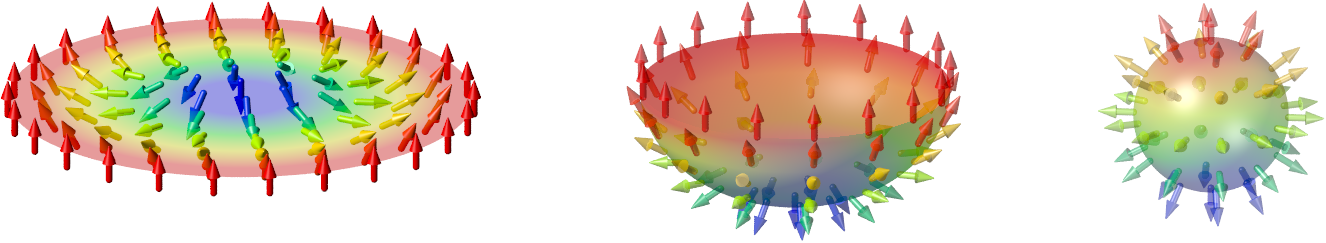
\includegraphics[width=0.39\linewidth]{hedgehog}
	\captionof{figure}[centering]{The wrapping of an anti-skyrmion configuration around the 2-sphere with $\mathcal{W} = -1$ \cite{Soccer}.}
\end{center}

A free electron travelling through a temporally or spatially inhomogeneous magnetic texture $\boldsymbol{\hat{M}}(\boldsymbol{r},t)$ is described by the Schr\"{o}dinger equation with Hamiltonian $H(\boldsymbol{r},t)$:
$$i\hbar \partial_{t}\ket{\chi} = \bigg[\frac{\boldsymbol{p}^{2}}{2m}\mathbb{1} + J\frac{g \mu_{B}}{2}\boldsymbol{\sigma}\cdot\boldsymbol{\hat{M}}(\boldsymbol{r},t)\bigg]\ket{\chi} = H(\boldsymbol{r},t)\ket{\chi}$$

for the two component spinor $\ket{\chi} = (\chi_{\uparrow},\chi_{\downarrow})^{T}$, with rows corresponding to majority and minority spin electrons respectively \cite{Soccer}.
}

%----------------------------------------------------------------------------------------
%	RESULTS 
%----------------------------------------------------------------------------------------

\headerbox{Results}{name=results2,span=2,column=1,below=results1,above=bottom}{ % To reduce this block to 1 column width, remove 'span=2'
In order to determine the motion of a free electron as a result of this Hamiltonian, we rotate the spin axis $\ket{\sigma}$ to align with $\boldsymbol{\hat{M}}(\boldsymbol{r},t)$, which may be achieved by the rotation matrix $U \propto \boldsymbol{\sigma} \cdot (\boldsymbol{\hat{M}}+\boldsymbol{\hat{e}}_{z})$ \cite{Morinari:2010wg}. The transformed Hamiltonian is then:$$i \hbar \partial_{t}\ket{\chi} = H\ket{\chi} \xrightarrow{U(\boldsymbol{r},t)} H'\ket{\psi} = \bigg[ q^{e}V^{e} + \frac{(\boldsymbol{p}\mathbb{1} - q^{e}\boldsymbol{A}^{e})^{2}}{2m} + J'\sigma_{z} \bigg]\ket{\psi}, \qquad \ket{\psi} = U(\mathbf{r},t)\ket{\chi}$$
where we have introduced the emergent scalar and vector potentials with an emergent charge $q^{e}$:$$V^{e} = -(i\hbar/q^{e}) U^{\dagger}\partial_{t}U, \qquad \boldsymbol{A}^{e} = (i\hbar/q^{e}) U^{\dagger}\grad U.$$In the adiabatic limit, we project these potentials onto the spin axis $\ket{\sigma}$ to determine that:$$\mathcal{V}_{\sigma}^{e} = \bra{\sigma}V^{e}\ket{\sigma} =  -(i\hbar/q^{e}) \bra{\Psi_{\sigma}}\partial_{t}\ket{\Psi_{\sigma}}, \qquad \boldsymbol{\mathcal{A}}_{\sigma}^{e} = \bra{\sigma}\boldsymbol{A}^{e}\ket{\sigma} =  (i\hbar/q^{e}) \bra{\Psi_{\sigma}}\grad \ket{\Psi_{\sigma}},$$
for $\ket{\Psi_{\sigma}} = U(\boldsymbol{r},t)\ket{\sigma}.$ These potentials can be identified with the famous Berry connection \cite{Berry45}, with the following Berry curvatures for each spin band $\sigma$ as emergent electric and magnetic fields:$$\boldsymbol{E}^{e}_{\sigma} = -\grad \mathcal{V}^{e}_{\sigma} - \partial_{t}\boldsymbol{\mathcal{A}}^{e}_{\sigma}, \qquad \boldsymbol{B}^{e}_{\sigma} = \grad \cross \boldsymbol{\mathcal{A}}^{e}_{\sigma}.$$
If $\boldsymbol{\hat{M}}(\boldsymbol{r},t) \equiv \boldsymbol{\hat{M}}(\boldsymbol{r})$, then it can be easily seen that $\boldsymbol{E}^{e} = 0$ and that:$$\boldsymbol{B}^{e}_{\sigma} = \mp\frac{2\mathcal{W}\hbar\lambda^{2}}{q^{e}(r^{2} + \lambda^{2})^{2}}\boldsymbol{\hat{e}}_{z} \equiv \pm\frac{\mathcal{W}\hbar}{2 q^{e}}\boldsymbol{\hat{M}}\cdot(\partial_{x}\boldsymbol{\hat{M}} \cross \partial_{y}\boldsymbol{\hat{M}})\boldsymbol{\hat{e}}_{z},$$
where $\boldsymbol{B}^{e}_{\sigma}$ is negative (resp. positive) for majority (resp. minority) spin electrons. It follows immediately that the surface integral over the skyrmion texture of $|\boldsymbol{B}^{e}_{\sigma}|$ is topologically quantised:$$\frac{1}{4\pi}\iint_{\text{skyrmion}}\boldsymbol{B}^{e}_{\sigma} \cdot\,d\boldsymbol{S} = \frac{-\mathcal{W}\hbar\lambda^{2}}{q^{e}}\int_{0}^{\lambda}\frac{r \,dr}{(r^{2} + \lambda^{2})^{2}} = -\mathcal{W}\hbar/2 q^{e}.$$
Now if we apply a magnetic field $\boldsymbol{B} = (0,0,-B)$ over the skyrmion, $\boldsymbol{\hat{M}}$ develops a time-dependence described by the dissipationless Landau-Lifshitz-Gilbert (LLG) equation \cite{Morinari:2010wg}:
$$\partial_{t}\boldsymbol{\hat{M}} = \alpha\boldsymbol{B}\cross\boldsymbol{\hat{M}} \quad \implies \quad \boldsymbol{\hat{M}}(\boldsymbol{r}, t) = \Big( \frac{2\lambda r}{r^{2} + \lambda^{2}}\cos\tilde{\Phi}(\phi,t), \frac{2\lambda r}{r^{2} + \lambda^{2}}\sin\tilde{\Phi}(\phi, t), \frac{r^{2} - \lambda^{2}}{r^{2} + \lambda^{2}}\Big),$$
where now $\tilde{\Phi}(\phi,t) = \mathcal{W}\phi - \alpha Bt + \phi_{0}$. The matrix $U(\boldsymbol{r},t)$ thus inherits this time-dependence, which lets us determine the new emergent electromagnetic fields; $\boldsymbol{B}^{e}_{\sigma}$ remains the same as before in the adiabatic limit, but now we have a nonzero $\boldsymbol{E}^{e}_{\sigma}$:$$\boldsymbol{E}^{e}_{\sigma} = \pm\frac{2\alpha B\hbar\lambda^{2}r}{q^{e}(r^{2} + \lambda^{2})^{2}}\boldsymbol{\hat{e}}_{r},$$
which acts in the positive (resp. negative) radial direction for majority (resp. minority) spin electrons. Hence we have found that the skyrmion texture gives rise to a spin-motive force that acts on free electrons, \textit{i.e.} the trajectory of the electron depends upon its spin state.


}

%----------------------------------------------------------------------------------------

\end{poster}

\end{document}